%\documentclass[review]{cvpr}
\documentclass[final]{cvpr}

\usepackage{times}
\usepackage{epsfig}
\usepackage{graphicx}
\usepackage{amsmath}
\usepackage{amssymb}

% Include other packages here, before hyperref.

% If you comment hyperref and then uncomment it, you should delete
% egpaper.aux before re-running latex.  (Or just hit 'q' on the first latex
% run, let it finish, and you should be clear).
\usepackage[pagebackref=true,breaklinks=true,colorlinks,bookmarks=false]{hyperref}


%\def\cvprPaperID{Project Proposal} % *** Enter the CVPR Paper ID here
%\def\confYear{CVPR 2021}
%\setcounter{page}{2} % For final version only


\begin{document}
\title{Deep Learning Project Proposal : Multi-instrument Classification using Partially Labeled Data and Weakly-supervised Learning}

\author{
	Clément Berger\\
	{\tt\small clement.berger@ensta-paris.fr}
% For a paper whose authors are all at the same institution,
% omit the following lines up until the closing ``}''.
% Additional authors and addresses can be added with ``\and'',
% just like the second author.
% To save space, use either the email address or home page, not both
\and Ilyes Er-Rammach\\
{\tt\small ilyes.er-rammach@ensta-paris.fr}

}

\maketitle
\begin{abstract}
	While single-instrument recognition has made tremendous progress, multi-instrument recognition is still considered as a hard task. A part of the difficulty comes from the lack of huge strongly labeled datasets. Recently, a large dataset of polyphonic audio clips called OpenMIC has been released. The drawback of the size of the dataset is that it is only weakly-labeled. Previous works have proposed to use an attention mechanism and a Recurrent Neural Network structure called Bidirectional Long-Short Term Memory (BiLSTM) to train on this dataset. Most works in this field use Log-Mel Spectrograms to treat the audio signal before giving it to the network. Here we explore the use of Analytic Wavelet Transform (AWT) to generate scalograms wich are then given to a Convolutional Neural Network (CNN). Such transformations are supposed to be more efficient in giving a representation of the whole signal. We also test different BiLSTM configurations and try some data augmentation techniques. While we do not improve state of the art, our results are encouraging. With more computational power, pretraining our scalogram-CNN structure as feature extractor using a big dataset like YouTube should be able to achieve great results.
\end{abstract}
\section{Introduction}
\subsection{Motivation}
Multi-instrument recognition is a subfield of Music Information Retrieval (MIR) in which, given a list of instruments and an audio clip, one tries to tell if these instruments figure in the clip or not. Such a task is very useful for music providers to make recommandations based on affinity with some instrument, or to create filters for research and so on. An efficient model could also be used as a basis (like a feature extractor) for other MIR tasks such that source separation, or music transcription.

Such a task requires not only machine learning skills, but also signal processing expertise. Great results have been achieved in single-instrument recognition, see e.g. \cite{mir}. However, polyphonic sounds are the superposition of multiple instruments with different charasteristics and played differently therefore most of these techniques can not be applied for our task.

Another challenge is the difficulty to create datasets. There are roughly two types of datasets of annotated polyphonic sounds. First there are small datasets but very strongly annotated. We can for example cite MusicNet \cite{MusicNet} containing 330 examples. Such datasets face big issues like overfitting. The other type of datasets is huge datasets (at least compared to the previous ones) but only partially labeled. In 2018 has been released a dataset called OpenMIC \cite{MIC} which belongs to the second category. OpenMIC contains 20 000 audio clips of 10 seconds, sampled at 44,1 kHz. However, given an audio clip, we only know if an instrument is in the clip or not but the offset et onset times are not provided. Practically this means that an audio containing 1 second of violin will have the same label as one completely played with a violin. Moreover, there are some missing labels, meaning that given an audio clip, some instrument labels are not provided. 
\subsection{Problem definition}
\subsubsection{Signal processing : different transformations}
We provide here a quick overview of two different transformations used in audio processing to create a visual representation of an a signal.

The first one is the genration of a Log-Mel Spectrogram. This is the result of a transformation based on the Short-Time Fourier Transform. The raw signal is divided into a certain number of overlapping frames, before applying a Fourier Transform on each frame. This result in a time frequency representation of the signal, using color variations to represent the magnitude of the Fourier Transforms. However, human sensibility is not homogeneous in frequencies. To account for this problem, we convert the Hertz into what is called a Mel scale \cite{mel}. It is a non linear transformation of the frequencies to get a scale which better describe human hearing. The resulting visual representation is called a Log-Mel Spectrogram. Such representations have been successfully used for music recognition, see e.g. \cite{spectrogram}.

The second one is the AWT used to generate a scalogram. Given a signal $x(t)$ and a wavelet $\psi(t)$ satisfying $\psi(t)=0$ for $t<0$, a function acting as a filter on the signal, the AWT of the signal is $AWT_{\psi}(t,s)=(1/2\pi)\int_0^\infty \bar{\psi}(s\omega)x(\omega)e^{j\omega}d\omega$. This is a variant of the Continuous Wavelet Transform comonly used in signal processing. We proceed as for the spectrogram to get a visual representation of this transform, which is then called a scalogram.
\subsubsection{VGGish network}
This section is devoted to briefly present a network created recently for multi-instrument recognition, called VGGish \cite{VGGish_net}. This name simply comes from the fact that it is derived from the classical VGG model \cite{vgg} used for image recognition. Amongst other changes, it has been modified to receive a Log-Mel Spectrogram as entry and the end of the network acts now as a compact embedding layer. A precise definition can be found \href{https://github.com/tensorflow/models/tree/master/research/audioset/vggish}{here}.
\subsubsection{F1-score}
For instrument classification, the performances of an algorithm are generally not measured in terms of the usual accuracy. Indeed, as some instruments are easier than others to recognize, a difference of accuracy doesn't perfectly reflect an improvement in the classification of hard instruments. Therefore, another metric called the F1 score has been created specificaly for this purpose \cite{metric}. 

We talk about true positive (TP) when both the network and the ground truth set the instrument as present in the audio. When the prediction is negative but should be positive, it is called a false negative (FN). There are similarly the false positive (FP) when the network predicts absence when it should not, and true negative when ground truth and network agree on the absence of the instrument. Then the precision (P) and recall (R) are introduced as :
\[P = \frac{TP}{TP+FP}\]
\[R=\frac{TP}{TP+FN}\]
Finally the F1-score is calculated as :
\[F1=\frac{2P\times R}{P+R}\]
\subsubsection{Training using OpenMIC}
In this work we try to train a network on the OpenMIC dataset for multi-instrument recognition. 

The OpenMIC dataset has been labeled with 20 instruments. For each of the 20 000 audio clips and each instruments, we have a binary value indicating if we have a label for this couple (audio, instrument) or not, and if we have so, we also have the probability that the instrument is effectively in the audio clip. In addition of the raw audios and labels, OpenMIC also provides features extracted using the VGGish. More precisely, a Log-Mel Spectrogram is computed for each raw audio, one frame corresponding to 1 second, and then given to the VGGish. After that, a Principal Component Analysis (PCA) is done on the extracted features for each frame. We end up with 10 vectors (one per second) containing 128 features, for each audio clip.
\section{Related work}
\subsection{Attention mechanism}
Multi-instrument recognition is not a new topic, and several works have been published. In 2018, Kong \etal \cite{kong} introduced an attention mechanism to train a CNN on another weakly-labeled dataset, AudioSet \cite{audioset}. This mechanism has then been used by Gururani \etal \cite{attention} on the OpenMIC dataset. Starting from the VGGish features furnished by OpenMIC, an embedding layer is then followed by a prediction layer coupled with the attention mechanism to produce the desired predictions. Let's describe briefly the attention mechanism. 

In Multi-Instance Label problems, a bag of labels is produced by a score function $S(X)=\mu(f(x)_{x\in X})$, where X is the input composed of multiple instances x, $f$ gives a prediction for each of these instances and $\mu$ aggregates these predictions to give the final prediction. The score (the global score $S$ as well as the instance-level scores $f$) represents in our case the probability of the label (here the probability for the instruments to effectively be part of the audio). Usually a max or an average is used for the aggregation function. However, previous works as Kong \etal \cite{kong} have shown that learning this function could lead to significant improvements. With this in mind, Gururani \etal parametrized this operator as :
\[S(X)=\sum_{x}w_xf(x)\]
with 
\[w_x =\frac{\sigma(v^{T}h(x))}{\sum_{x'}\sigma(v^{T}h(x)')}\]
where $h(x)$ is the output of the embedding layer, $v$ is a vector to be learned, and $\sigma$ is the sigmoid function. Note that the division is here to enforce the sum of coefficients to be 1. The formula also means that the attention layer takes as input the results of the embedding layer and then use this information to aggregate the results of the prediction layer represented by $f$.
\subsection{Using a BiLSTM architecture}
In 2020, Amir Kenarsari-Anhari \cite{squelette_progr} built upon these works to improve the efficiency of the network introduced in the previous section. His idea was to use Recurrent Neural Networks (RNN) to better exploit the fact that the different vectors of features correspond to different seconds of the audio clip (as explained in the Section 1.2.1). In particular, he used a BiLSTM structure. An LSTM is a particular structure of RNN built especially to improve the ability of the network to pass information through time, which has proved its efficiency in Natural Language Processing or to study Time Series (see \cite{lstm} for a complete description). It is here set to be bidirectional in the sense that it treats the data by following the its direction as well as reversing it.

Practically, the BiLSTM replaced the embedding and prediction layers used by Gurarani \etal to be coupled with the attention mechanism. The resulting architecture, presented in figure \ref{mel}, improved the efficiency of the model and will be considered as the state of the art for us. 
\subsection{Using scalograms}
In 2020, a paper from Dutta \etal \cite{features_descr} investigated the use of scalograms based on AWT using a Morse wavelet to replace the spectrograms, for \textit{single}-instrument recognition. The problem of the spectrograms using STFT is that as the signal is cut in pieces before processing each part independently, it is harder to get back the unity of the signal. That is a particular issue in our case as we do not have the onset and offset times of the instruments. This means that some pieces of the signal (after cutting) are treated as if they were containing an instrument while they may not. This procedure also significantly looses efficiency when the signal contains very low or very high frequencies. 

On the contrary, the AWT is computed over the whole signal. Therefore is supposed to be able to extract features taking into account the entire audio clip, which should thus be better.

The generated scalograms have been given to a CNN to extract the extract the features, ending with a classification layer. Used to distinguish 14 different instruments, the model achieved a reasonnable accuracy and is to be followed by further works on the topic.
\subsection{Data augmentation}
As told before, a big issue in MIR can be the absence of a big dataset corresponding to a given task. Naturally researchers have been working on different data augmentation techniques, general or specified for a task. We can cite Schütler and Grill \cite{data_aug} who proposed to randomly add a Gaussian noise to slightly modify the data. 

Zhang \etal \cite{interpol} experimented interpolation between different samples. More precisely, given $\lambda\in[0,1]$ and two signals x and y, labeled by $l_x$ and $l_y$, we create a new signal $z$ with the label $l_z$ by computing :
\[z = \lambda x+(1-\lambda)y\]
\[l_z = \lambda l_x+(1-\lambda)l_y\]
\section{Methodology}
\subsection{BiLSTM}
\subsection{Spectorgrams}
\subsection{Data augmentation}
\begin{figure}
	\centering
	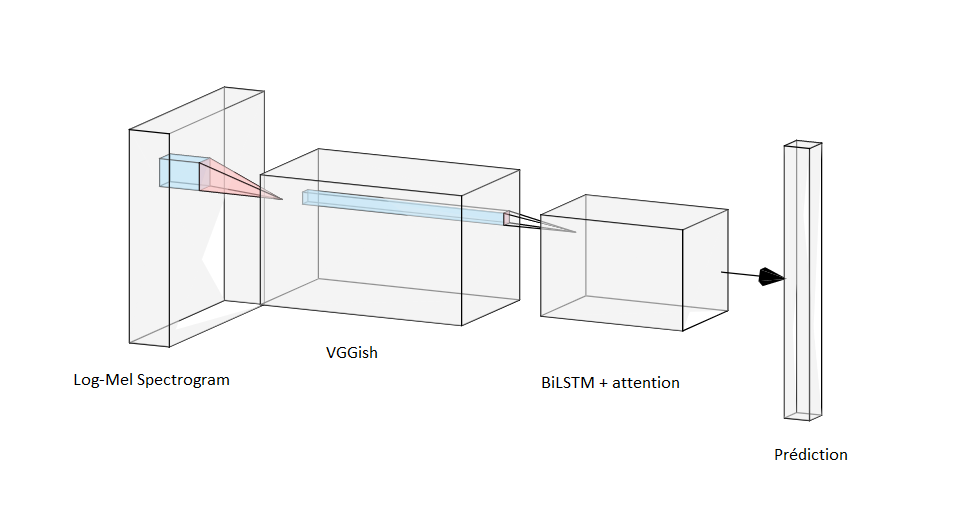
\includegraphics[scale = 0.45]{bilstm.png}
	\caption{Structure using Log-Mel Spectrogram}
	\label{mel}
\end{figure}
\begin{figure*}
	\centering
	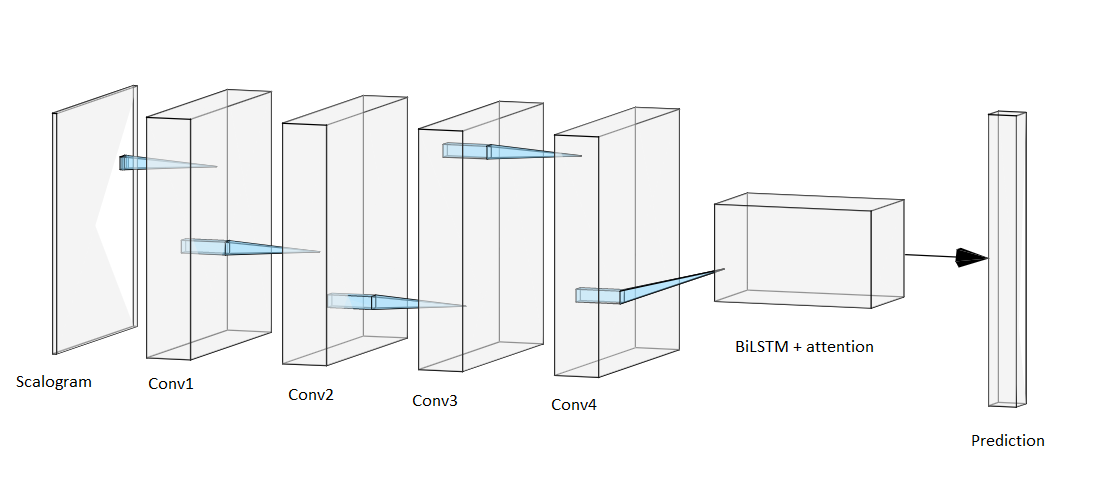
\includegraphics[scale = 0.65]{cnn.png}
	\caption{Convolutional network taking scalograms}
	\label{cnn}
\end{figure*}
\begin{figure}
	\centering
	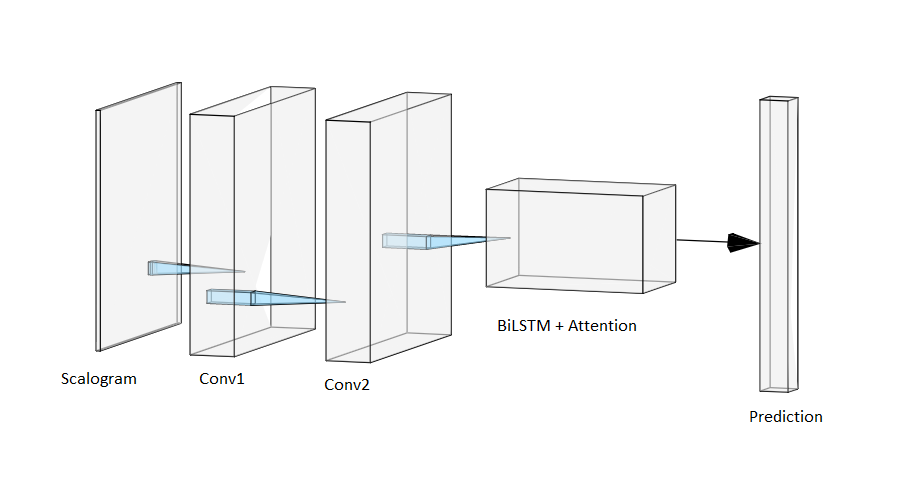
\includegraphics[scale = 0.45]{cnnreduit.png}
	\caption{Convolutional network taking scalograms, reduced structure}
	\label{reduit}
\end{figure}
\begin{figure}
	\centering
	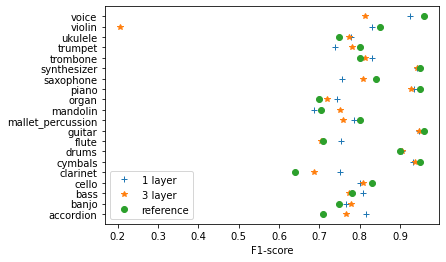
\includegraphics[scale = 0.5]{to_ref.png}
	\caption{Comparison of the instrument-level F1-score between our different Mel architectures and state of the art (denoted by \textit{reference}), with no data augmentation.}
	\label{to_ref}
\end{figure}
\begin{figure}
	\centering
	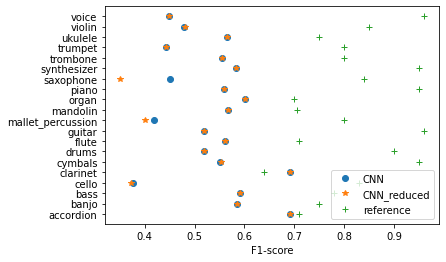
\includegraphics[scale = 0.5]{cnn_plot.png}
	\caption{Comparison of the instrument-level F1-score between our Mel 1-layer architecture and our CNN and CNN-reduced architectures, with no data augmentation.}
	\label{cnn_plot}
\end{figure}
\begin{figure}
	\centering
	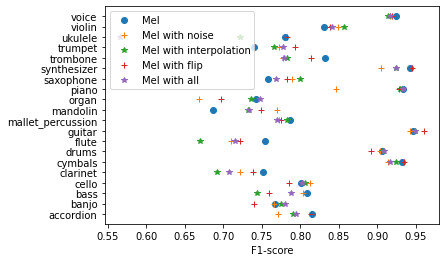
\includegraphics[scale = 0.5]{mel_data.png}
	\caption{Comparison of the instrument-level F1-score between our different data augmentation strategies for the 1-layer Mel structure.}
	\label{mel_data}
\end{figure}
\begin{figure}
	\centering
	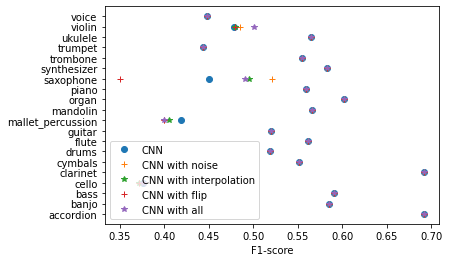
\includegraphics[scale = 0.5]{cnn_data.png}
	\caption{Comparison of the instrument-level F1-score between our different data augmentation strategies for the CNN structure.}
	\label{cnn_data}
\end{figure}
\section{Evaluation}

{\small
	\bibliographystyle{ieee_fullname}
	\bibliography{report}
}
\end{document}